%! Licence = CC BY-NC-SA 4.0

%! Author = gianfluetsch
%! Date = 22. Jan 2022
%! Project = icth_summary

\section{Quadrature Amplitude Modulation (QAM)}

\subsubsection{A}
Ein binärer Datenstrom soll via eine 64-QAM Modulation über ein verdrilltes Kupferaderpaar übertragen werden.\\
In der unterstehenden Signalebene sind die Signalpunkte eingetragen.Wie gross ist der Abstand jedes Signalpunktes von der nächsten Entscheidungsschwelle?\\
\begin{center}
    \vspace{-8pt}
    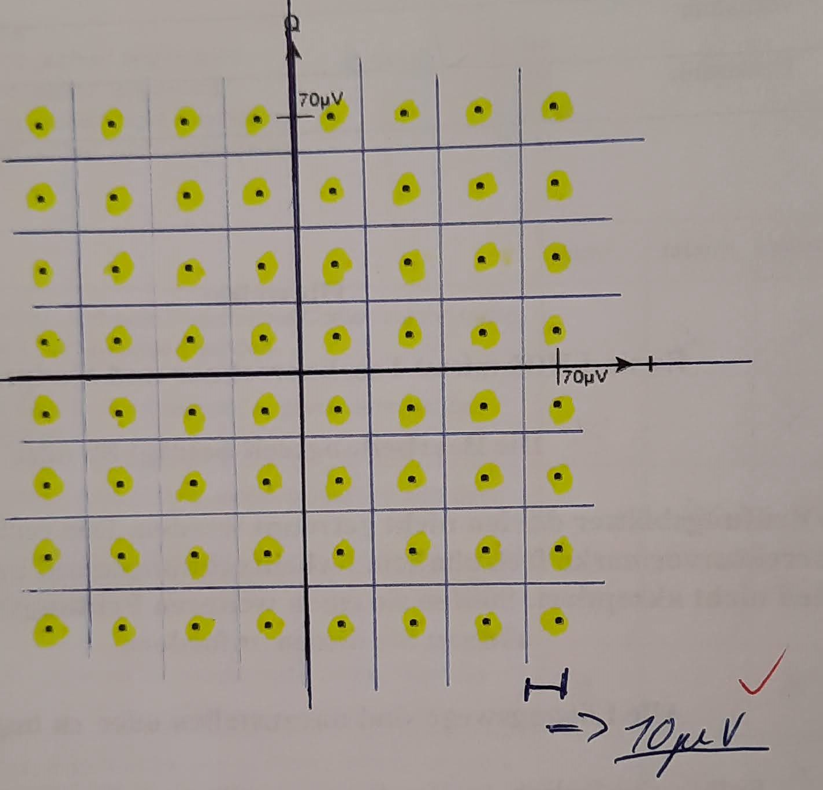
\includegraphics[width=.5\linewidth]{./07-qam/hs2020-2}
    \vspace{-8pt}
\end{center}

\textbf{Wie gross wird bei $U_{eff}=1\mu V$ (entspricht einer Bitfehlerrate $BER = 10^{-23}$) die mittlere Rauschleistung N in [W] an einem Widerstand von $R=100\Omega$? 
Drücken Sie diese Rauschleistung auch als N in [dBm] aus.}\\
$N=\frac{(U_{eff})^2}{R}=\frac{(1'-{-6})^2}{100\Omega} \rightarrow 10^{-4}W=0.01pW$\\
$10*log_{10}(\frac{10^{-14}}{10^{-3}})=10*log(10^{-11})=-110dBm$

\subsubsection{B}
Ein binärer Datenstrom soll via eine 64-QAM Modulation über ein verdrilltes Kupferaderpaar mit Wellenimpedanz $Zw = 100 \Omega $  übertragen werden.\\
In der unterstehenden komplexen Signalebene sind die vier Signalpunkte mit der grössten Leistung eingetragen. Ergänzen Sie das 64-QAM Modulationsschema und zeichnen Sie
die Entscheidungsschwellen ein.\\
\begin{center}
    \vspace{-8pt}
    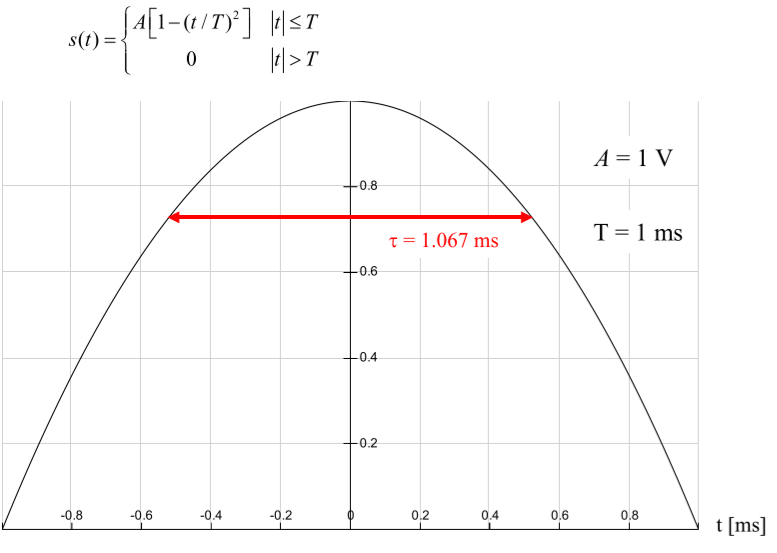
\includegraphics[width=.5\linewidth]{./07-qam/hs2019}
    \vspace{-8pt}
\end{center}

\textbf{Wie gross ist der Abstand jedes Signalpunkts von der nächsten Entscheidungsschwelle?}\\
$50\mu V$\\

\textbf{Welchen Effektivwert $U_{eff}$ darf das normalverteilte Rauschen haben, wenn das Signal-zu-Rauschverhältnis \textbf{SNR = 20 dB} sein soll, damit eine Bitfehlerrate \textit{$BER = 10^{-23}$} resultiert?}\\
$1\mu V$\\

\textbf{Wie gross wird beim oben bestimmten Ueff die mittlere Rauschleistung N in [W] an einem Widerstand von $R = 100 \Omega$? Drücken Sie diese Rauschleistung auch als N in [dBm] aus.}\\
$N=\frac{U_{eff}^2}{R}=\frac{(10^{-6})^2}{100}=10^{-14}W=0.01pW$\\
$N=10log_{10}\frac{N}{10^{-3}}=10log(10-{-11})=-110dBm$\\

\textbf{Da es sich um weisses Rauschen handelt, gilt $N=10logkT\Delta f=-174dBm+10log\Delta f$.
Wie gross darf die Systembandbreite B maximal sein, damit der oben berechnete Rauschpegel für die 64-QAM Detektion nicht überschritten wird?}\\
$10logB=N+174dBm=-110dBm+174dBm=64dB$\\
$\rightarrow$ Systembandbreite: $B=10Mhz/4=2.5MHz$\\

\textbf{Wie hoch darf die Bitrate des mit 64-QAM modulierten Datenstroms maximal sein, damit die Bitfehlerrate \textbf{$BER = 10^{-23}$} eingehalten wird?}\\
Da mit 64-QAM 6 Bit pro Symbol übertragen werden können, resultiert eine Bitrate von 15 Mbit/s.\\
Weil B=2.5MHz $\rightarrow$ Symbolrate max 2.5MBaud, da 64 QAM (also 6 Bit pro Symbol) $\rightarrow$ Bitrate von 15Mbits/s (2.5 MBaud*6Bit).\\
Wegen der vorgegebenen Systembandbreite von B = 2.5 MHz darf die Symbolrate maximal 2.5 MBaud sein.

